\chapter{Vectors and Matrices}
You've come a long way in your problem solving journey. You've used algebra to solve simple equations like $7x + 10 = 24$ and quadratic equations like $4x^{2} + 9x + 31 = 0$. Algebra works with scalars, regular numbers that represent values. You also learned about vectors, quantities that represent both a magnitude and direction. Recall the parachute jumper in Workbook 5. To figure out the force, and in turn how fast the parachutist is traveling, you needed to know the direction and speed of the wind, the direction and speed of the plane, the wind resistance, and gravity. A scalar can represent speed, but to take direction into account, you need to use vectors. That's where linear algebra comes in.    

Linear algebra is a specialized form of algebra that represents and manipulate linearly related variables. It uses vectors and matrices to represent variables. A vector is a one-dimensional array of numbers. A matrix is a multidimensional array of numbers. In this chapter, a matrix will be two dimensions. You can think of a matrix as a collection of vectors. 

As you work through this module, you’ll see that you already know the fundamentals (vectors, scalars, dot products) and how to apply these concepts to practical problems. You’ve also had some experience with matrices in the form of spreadsheets. 

Matrices can represent:
\begin{itemize}
\item A linear transformation, such as rotation, scaling, and skewing. You apply a transformation to a vector by multiplying the vector by a matrix.  
\item A system of linear equations. Linear algebra provides various methods that you can use to find the solution vector. 
\end{itemize}

\section{Applications of Matrix-Vector Multiplication}
Many areas in engineering and science rely on matrix-vector multiplication. These are just a few examples. As you encounter more topics in science and engineering, you will find that matrix-vector multiplication is crucial to many other fields.
\subsection{Computer Graphics}
When you play a video game or watch the latest CG animation, matrix operations transform objects in the scene to make them appear as if moving, getting closer, and so on. You can represent the vertices of objects as vectors, and then apply a transformation matrix.
\subsection{Data Analysis}
We live in an era in which it's easy to collect so much data that it's difficult to make sense of the data by just looking at it. You can represent the data in matrix form and then find a solution vector. For example, scientists use this technique to figure out the effectiveness of drug treatments on disease.
\subsection{Economics}
Take a look at financial section of any news organization and you'll see headlines such as "Economic Data Points to Faster Growth" or "Is the Inflation Battle Won?" Economists can use systems of linear equations to represent economic indicators, such as consumer consumption, government spending, investment rate, and gross national product. By using various methods that you'll learn about later, they can get a good idea of the state of the economy.
\subsection{Engineering}
Engineering couldn't do without vector-matrix multiplication. For example, the orbital dynamics of space travel relies on it. Engineers must predict and calculate the the motion of planetary bodies, satellites, and spacecraft. By solving systems of linear equations engineers can make sure that a spacecraft travels to its destination without running into a satellite or space rock.
\subsection{Image Processing}
An image is a matrix of pixel values. When you take a selfie and apply a filter, the image app applies a transformation to the image matrix. A simple operation would be to change the tint of the image. A more complex operation would be to skew the image to make it distorted, like a funhouse mirror.

\section{Let's Observe the Sun!}
India recently sent the Aditya spacecraft on a mission to study the Sun. Without a thorough understanding of vectors, the engineers would not have accomplished the amazing feat of getting Aditya in a stable orbit around a Lagrange point. In previous chapters you learned about gravity and its effects. 

A Lagrange point is a point in space between two bodies (e.g. Earth and Sun) where there is gravitational equilibrium. With the right trajectory, a spacecraft will orbit around a Lagrange point in a stable position that doesn’t require much energy to maintain. That’s called a Halo orbit. Because that there are no fueling stations in space, a Halo orbit will allow Aditya to maintain position for about 5 years. Pretty good mileage!

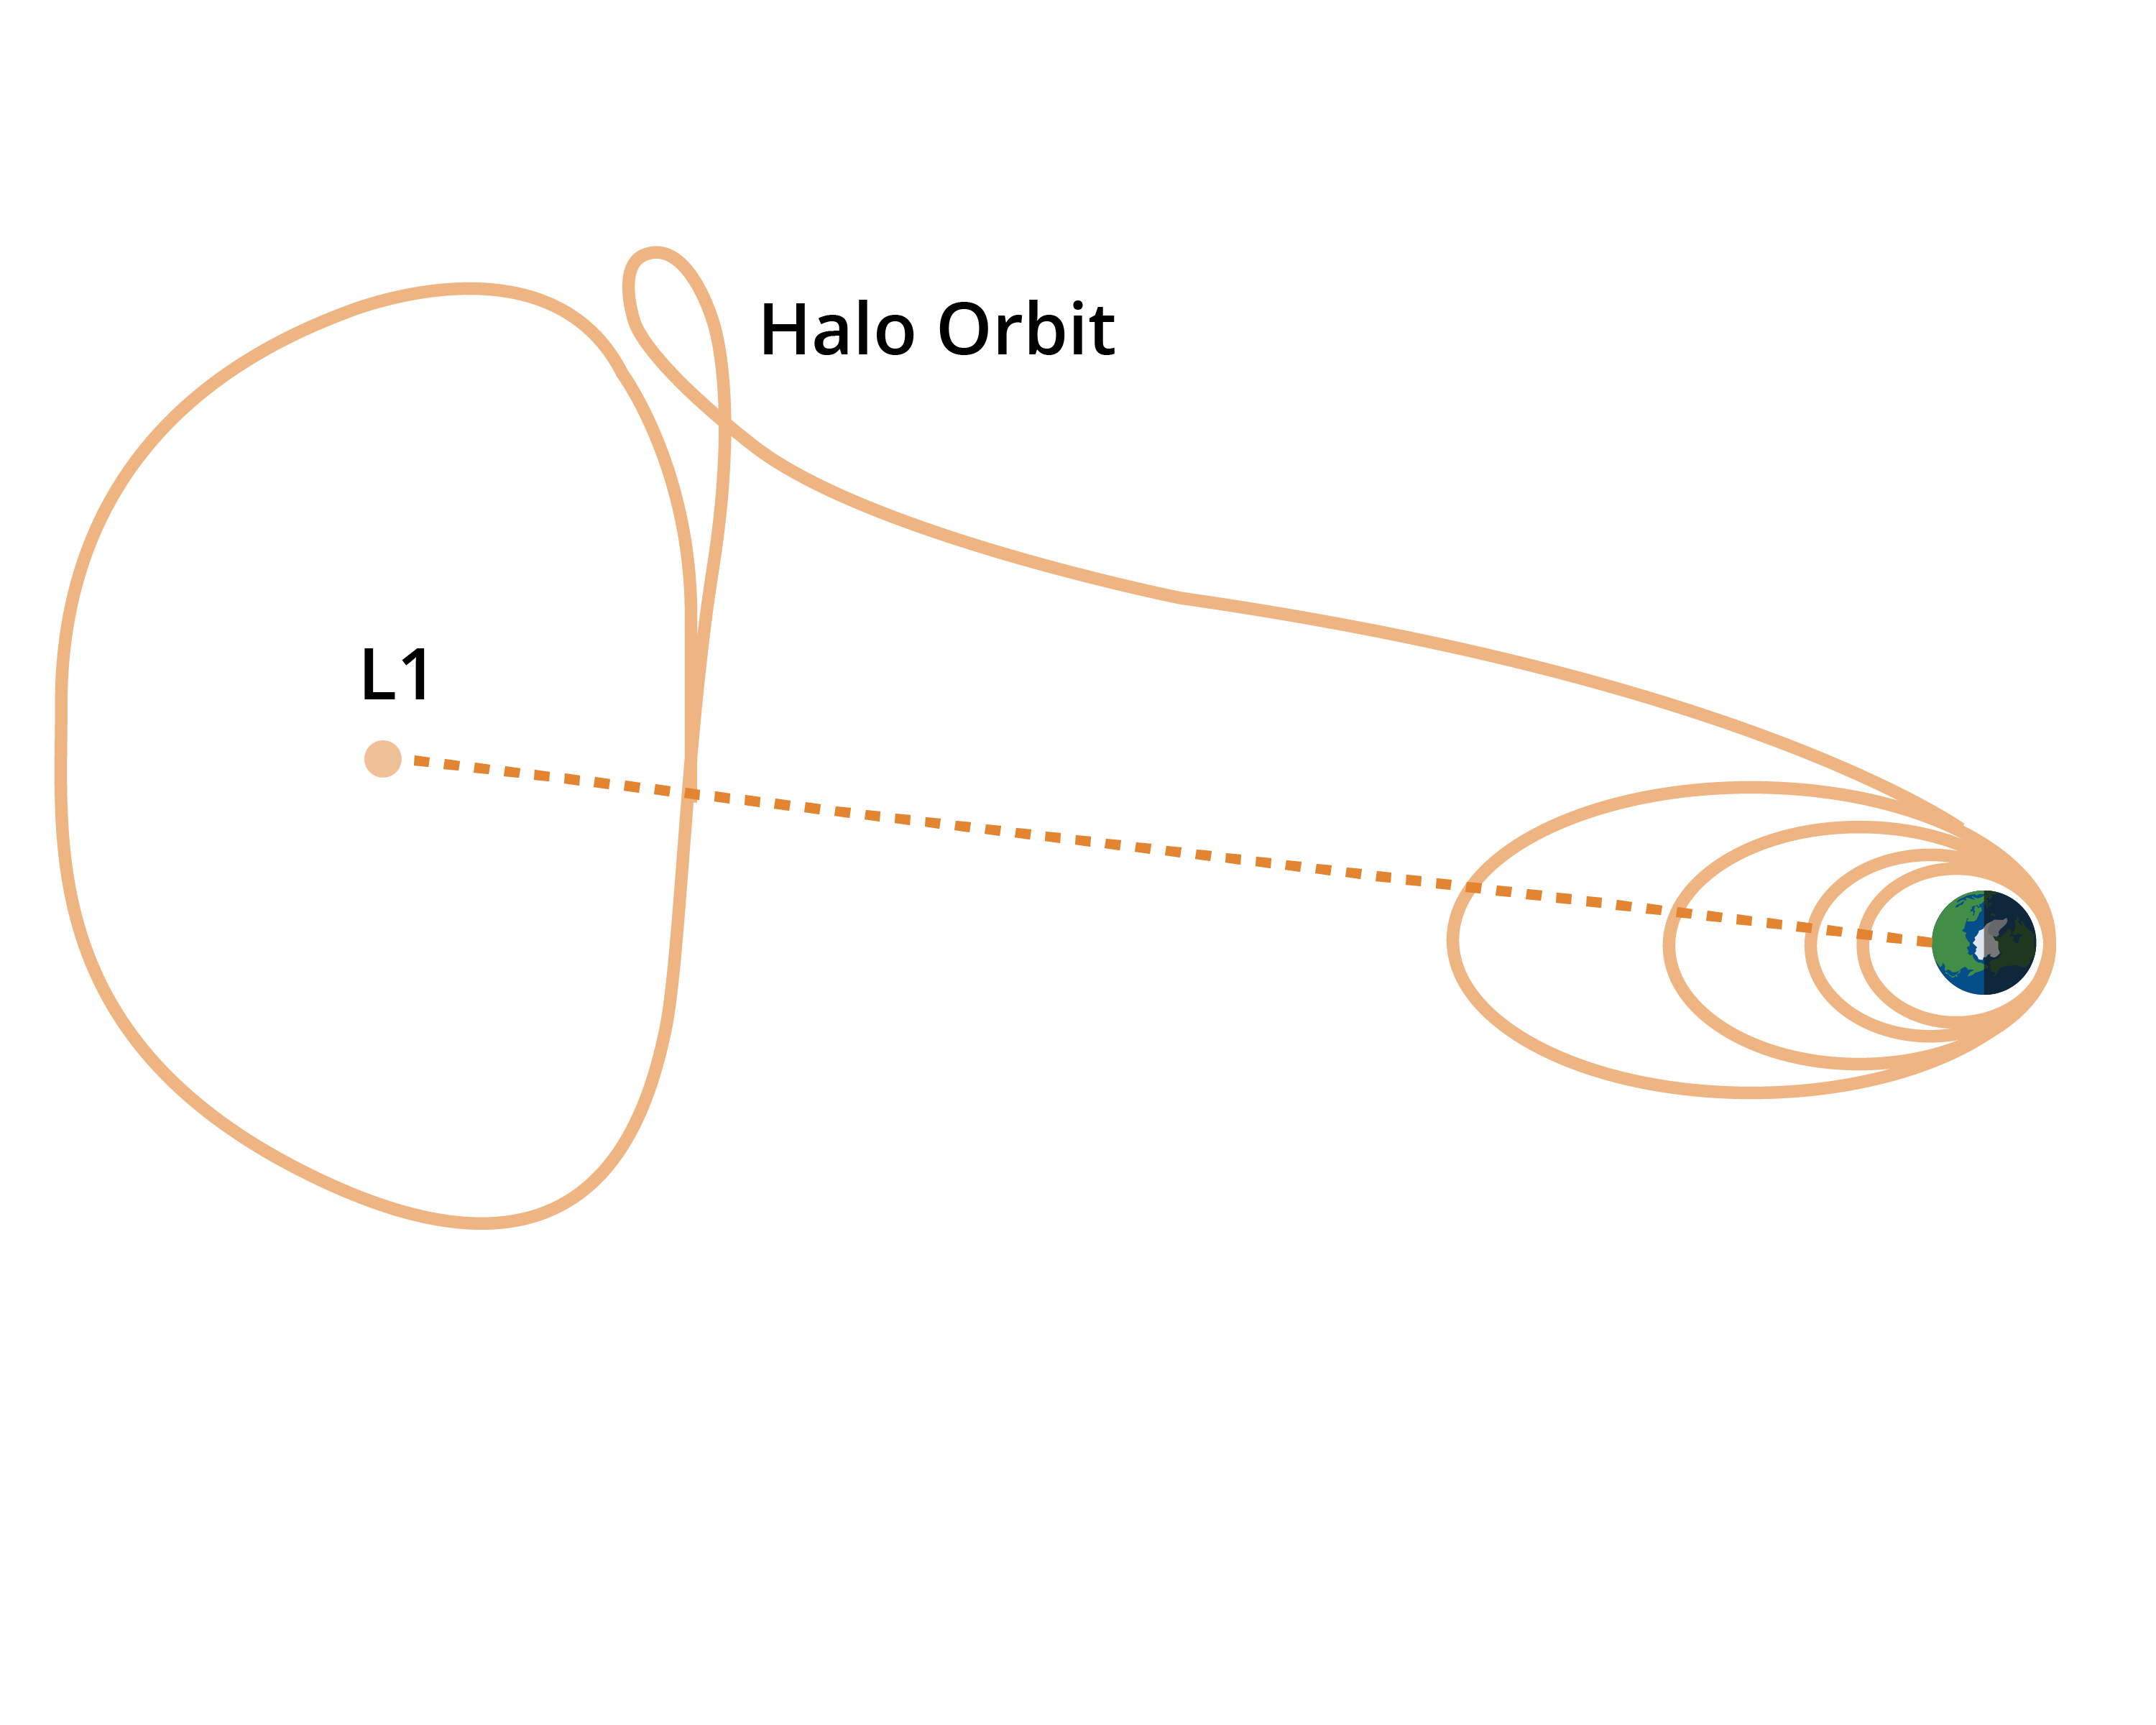
\includegraphics[width=0.5\textwidth]{orbit.png}

Aditya’s engineers had to calculate a looping maneuver that would precisely inject the Aditya spacecraft into the Halo orbit. They determined the angles and burn times for the thrust engine. If they were wrong in one direction, the spacecraft would fly off to the sun. The other direction would send the spacecraft back in the direction of Earth. Their success is due to a solid understanding of vectors and linear algebra.

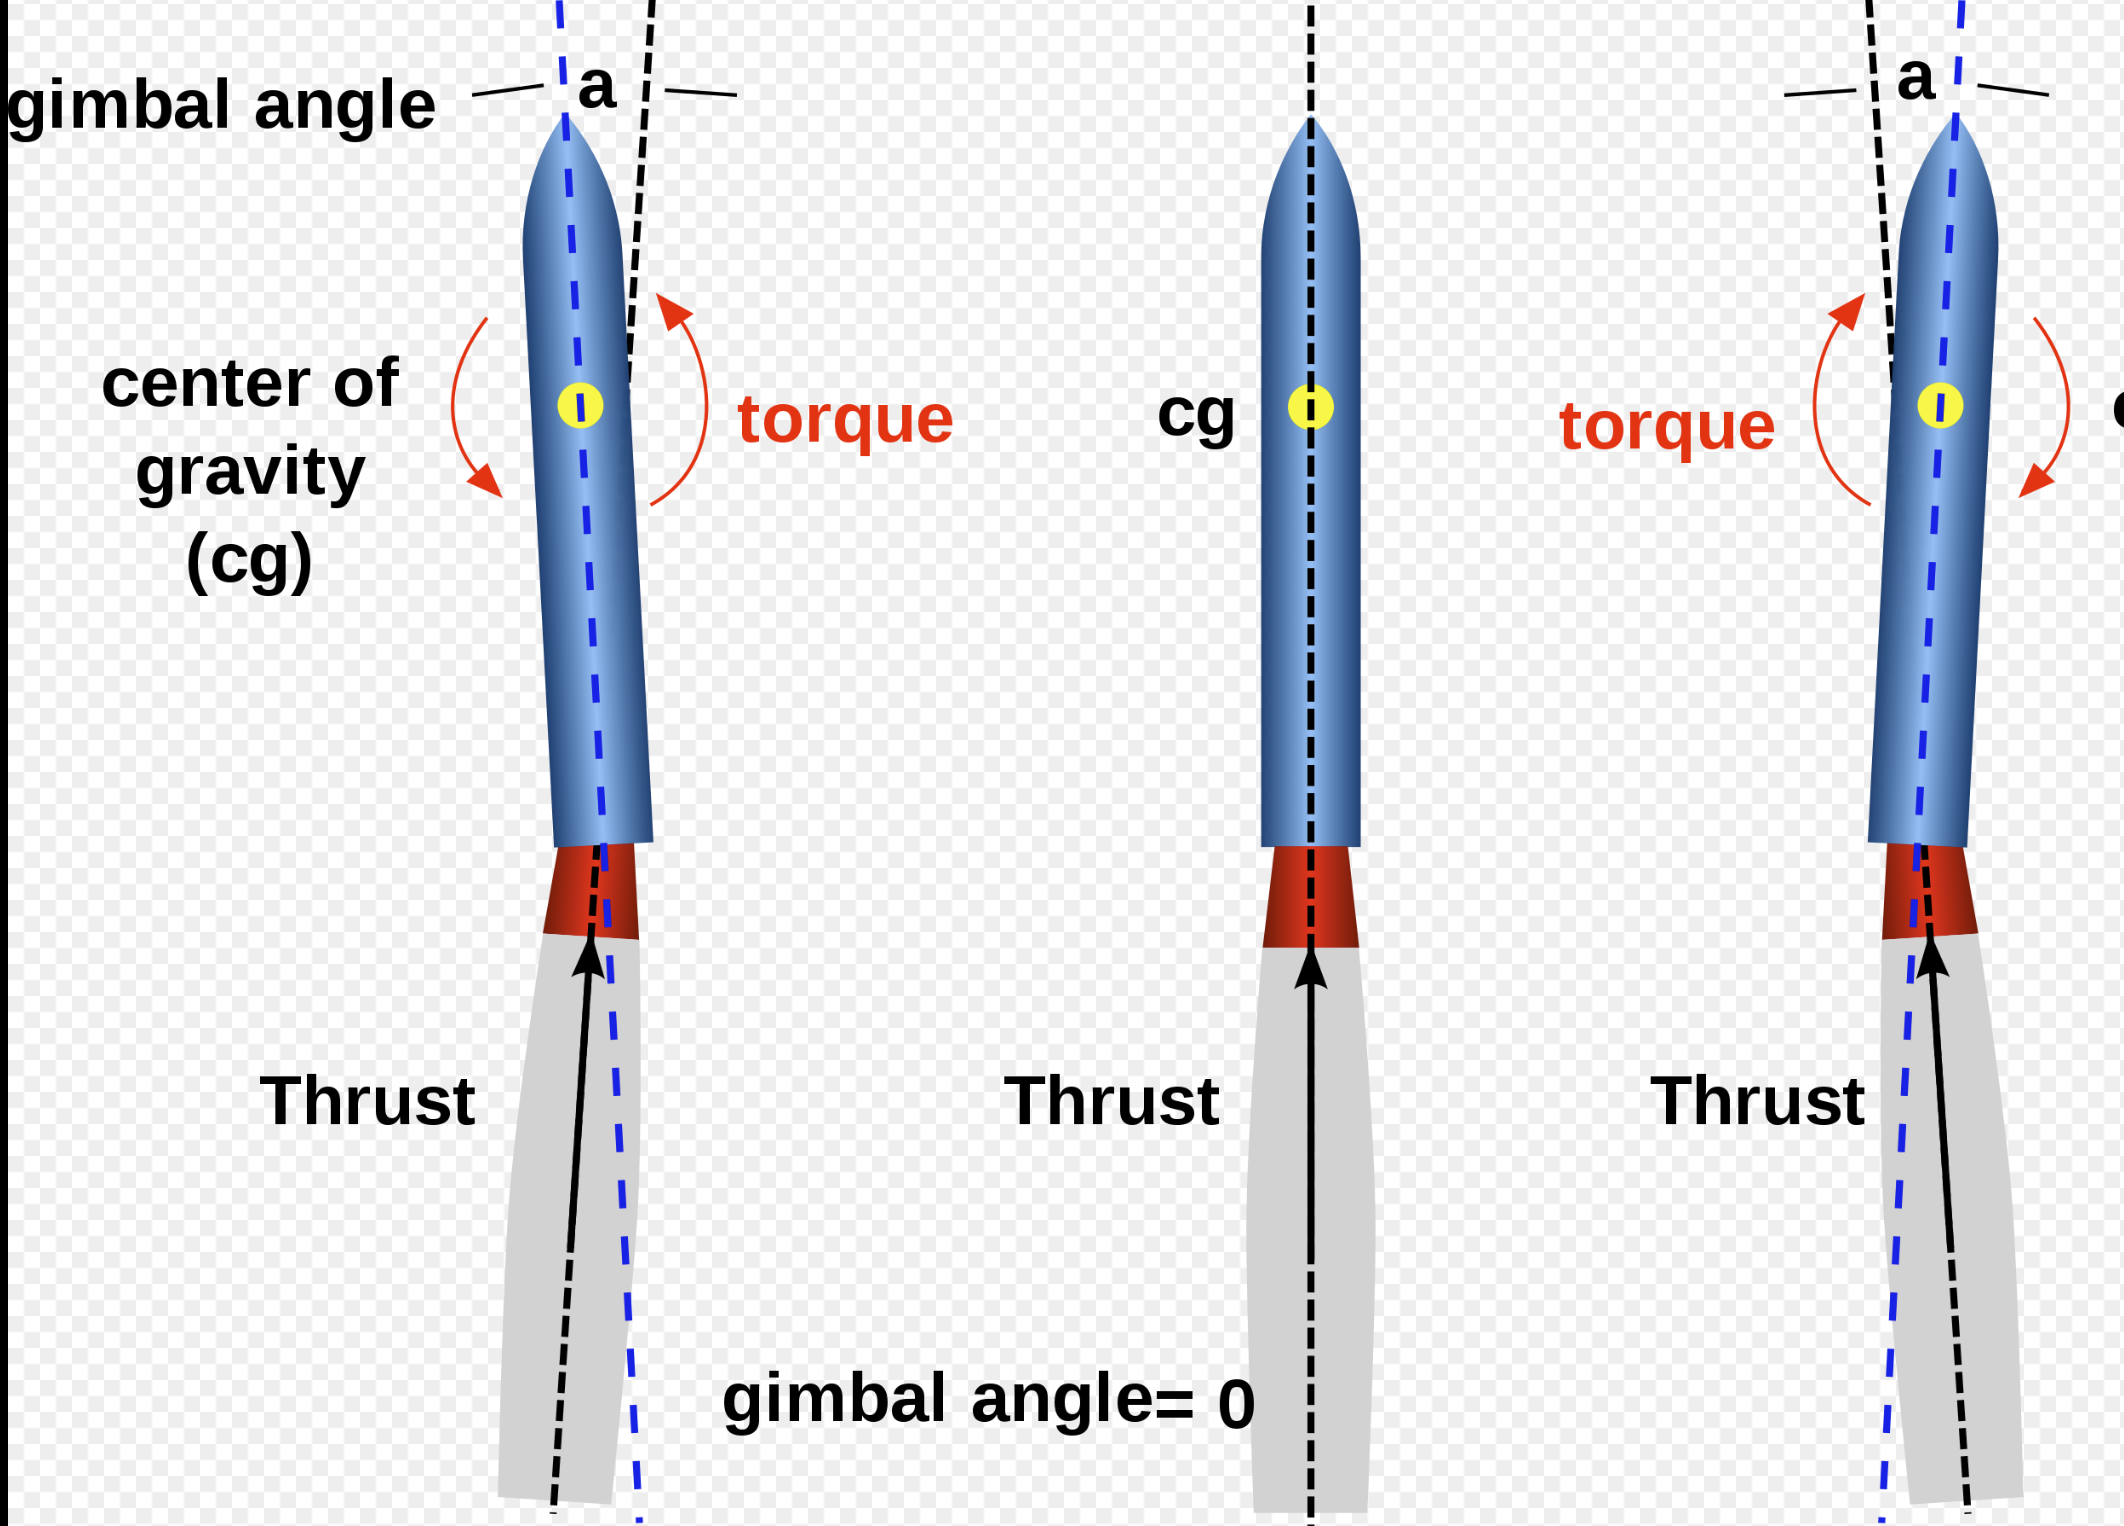
\includegraphics[width=0.5\textwidth]{thrust.png}

\section{Vector-Matrix Multiplication}
Let's take a look at the general form of vector-matrix multiplication. Given a matrix $A$ of size $m \times n$ and a vector $x$ of size $n \times 1$, the product $Ax$ is a new vector of size $m \times 1$. 

You compute the $i$-th component of the product vector $Av$ by taking the dot product of the $i$-th row of $A$ and the vector $v$:

\begin{equation*}
(Av)_i = \sum_{j=1}^n a_{i,j}x_j
\end{equation*}

where $a_{i,j}$ is the element in the $i$-th row and $j$-th column of $A$, and $v_j$ is the $j$-th element of $v$.

This is the general form of a matrix and a vector, written to show the specific components of each:


 $$A = \begin{bmatrix}
 a_{1,1} & a_{1,2}  & a_{1,3} & ... & a_{1,n}  \\
 a_{2,1} & a_{2,2}  & a_{2,3} & ... & a_{2,n}  \\
 ... \\
 a_{m,1} & a_{m,2}  & a_{m,3} & ... & a_{m,n}  
\end{bmatrix}$$

$$v = \begin{bmatrix}
 v_{1}  \\
 v_{2} \\
 v_{3} \\
 ... \\
 v_{m} 
\end{bmatrix}$$

 $$Av =\begin{bmatrix}
 v_{1}*a_{1,1} +v_{2}*a_{1,2}  +v_{3}*a_{1,3} +... +v_{m}*a_{1,n}  \\
 v_{1}*a_{2,1} +v_{2}*a_{2,2}  +v_{3}*a_{2,3} +... +v_{m}*a_{2,n}  \\
 ... \\
 v_{1}*a_{m,1} +v_{2}*a_{m,2}  +v_{3}*a_{m,3} +... +v_{m}*a_{m,n}  
\end{bmatrix}$$

Let's look at a specific example.

$$A = \begin{bmatrix}
 2  & 4 & 6  \\
 3  & 5 & 7  \\
 1  & 2 & 3  \\
 8  & 6 & 2 
\end{bmatrix}$$

$$v = \begin{bmatrix}
 -2  \\
 1 \\
 3 
\end{bmatrix}$$

Solution:
$$= \begin{bmatrix}
-2*2+1*4+3*6\\
-2*3+1*5+3*7\\
 -2*1+1*2+3*3\\
-2*8+1*6+3*2
\end{bmatrix}$$

$$= \begin{bmatrix}
18 \\
20\\
9\\
-4 
\end{bmatrix}$$
$$= (18,20,9,-4)$$

\begin{Exercise}[title={Vector Matrix Multiplication}, label=vector-matrix-multiply01]
Multiply the array $A$ with the vector $v$. Compute this by hand, and make sure to show your computations. 
$$A = \begin{bmatrix}
1 & -2  & 3 & 5  \\
-4  & 2  & 7 & 1 \\
3  & 3  & -9 & 1
\end{bmatrix}$$
	$$v = 
	\begin{bmatrix}
		2 \\
 		2 \\
 		6 \\
 		-1
	\end{bmatrix}$$
\end{Exercise}
\begin{Answer}[ref=vector-matrix-multiply01]
$$Av = (11 37 -43)$$
\end{Answer}

\subsection{Vector-Matrix Multiplication in Python}
Most real-world problems use very large matrices where it becomes impractical to perform calculations by hand. As long as you understand how matrix-vector multiplication is done, you'll be equipped to use a computing language, like Python, to do the calculations for you. 

Create a file called \filename{vectors\_matrices.py} and enter this code:

\begin{Verbatim}
// import the python module that supports matrices
import numpy as np

// create an array
a = np.array([[5, 1, 3, -2], 
              [1, -1, 8, 4], 
              [6, 2, 1, 3]])

// create a vector 
b = np.array([1, 2, 3, -8])

//calculate the dot product
print(a.dot(b))
\end{Verbatim}

When you run it, you should see:
\begin{Verbatim}
[16, 6, 8]
\end{Verbatim}

\section{Where to Learn More}
Watch this video from Khan Academy about matrix-vector products: \url{https://rb.gy/frga5}

